Classic optical properties question.

\begin{parts}
	\part Standard derivation.
	You really should know how to do this off your head by the time you read this.
	
	\textit{Anyway standard answers below:}
	
	As usual, to find relative permittivity $\epsilon_r$ we shall imagine the system as a collection of electric dipoles $\longrightarrow$ \textit{find displacement $\mathbf{x}$ first!}
	
	Plugging in Ansatz $\mathbf{x} = \mathbf{x}_0 \exp\sbracket{i(\mathbf{k}\cdot\mathbf{r}-\omega t)}$ gives
	\begin{gather*}
		-m\omega^2 \mathbf{x}_0 -im\gamma\omega \mathbf{x}_0 = q\mathbf{E}_0 \\
		\Rightarrow \mathbf{x}_0 = \frac{q\mathbf{E}_0}{-m\omega^2 -im\gamma\omega}
	\end{gather*}
	where $\gamma = \tau^{-1}$.
	
	Next we find polarisation $\mathbf{P} = Nq\,\mathbf{x}$, combining this together with the definition of the displacement field $\mathbf{D} = \epsilon_0\mathbf{E} + \mathbf{P} + \mathbf{P}_\textnormal{bg} = \epsilon_0 \epsilon_r \mathbf{E}$, where $\mathbf{P}_\textnormal{bg}$ is the background polarisation, then gives
	\begin{align*}
		\epsilon_r &= 1 + \chi_\textnormal{bg} + \frac{Nq\,\mathbf{x}}{\epsilon_0 \mathbf{E}} \\
		&= 1 + \chi_\textnormal{bg} + \frac{Nq\,\mathbf{x}_0}{\epsilon_0 \mathbf{E}_0} \\
		&= \underbracket{1 + \chi_\textnormal{bg}}_{\epsilon_\infty} + \frac{Nq^2}{\epsilon_0 \rbracket{-m\omega^2 -im\gamma\omega}} \\
		&= \epsilon_\infty + \frac{\epsilon_\infty \omega_p^2}{-\omega^2 - i\gamma\omega} \\
		&= \epsilon_\infty \rbracket{1 - \frac{\omega_p^2}{\omega^2 + i\omega/\tau}}
	\end{align*}
	where $\omega_p^2 = \dfrac{Nq^2}{m\epsilon_0 \epsilon_\infty}$ is the plasma frequency.
	
	\part Lookup from the graph to get $N$. I picked the high-frequency limit so $\epsilon_r \rightarrow \epsilon_\infty \rbracket{1 - \omega_p^2/\omega^2}$.
	
	Then we have reflectivity $R$ with the complex refractive index $\tilde{n} = \sqrt{\epsilon_r}$:
	\begin{equation}
		R = \abs{\frac{\tilde{n} - 1}{\tilde{n} + 1}}
		\label{eqn:q3-reflectivity}
	\end{equation}
	
	Rearranging \eqref{eqn:q3-reflectivity} gives
	\begin{equation}
		\abs{\epsilon_r} = \abs{\frac{1 + R}{1 - R}}^2
	\end{equation}
	
	\newpage
	Plugging in $R=0.05$, $\hbar\omega = \SI{21}{\electronvolt}$, and $\epsilon_\infty = 1$ due to aluminium being metal (or from the graph $R(\omega\rightarrow\infty)=0$) gives
	\begin{gather*}
		\abs{1-\frac{\omega_p^2}{\omega^2}} = \abs{\frac{1 + R}{1 - R}}^2 \\
		\Rightarrow \frac{\omega_p^2}{\omega^2} = \abs{\frac{1 + R}{1 - R}}^2 + 1 \textnormal{\hspace{1em}by inspection} \\
		\omega_p^2 = \SI{2.26e33}{\radian\per\second}
	\end{gather*}
	
	Further plugging in $q=e$, $m=m_e$ into the definition of $\omega_p$ then give
	\begin{equation*}
		N = \omega_p^2 \times \frac{m_e \epsilon_0}{e^2} = \SI{7.11e29}{\per\metre\cubed}
	\end{equation*}
	
	\begin{figure}[H]
		\centering
		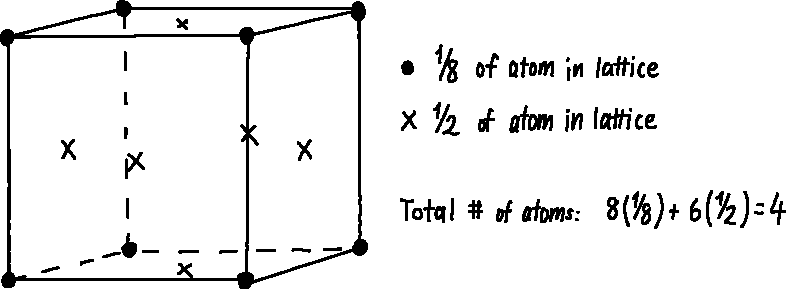
\includegraphics[width=.6\linewidth]{q3-fcc}
	\end{figure}
	
	Then we realise that in an FCC lattice, the carrier density is
	\begin{equation}
		N = \frac{4x}{a^3}
		\label{eqn:q3-fcc-density}
	\end{equation}
	where $x$ is the valency\footnote{Is this really valency though? I think my chemist friends would fill my inbox with friendly reminders that aluminium has a valency +3, the $x$ I calculated here is the atomic number I believe.} of aluminium.
	
	Solving \eqref{eqn:q3-fcc-density} then gives $x=11.8$.
	
	\part The magnitude of the energy suggests that the dip is due to a band transition\footnote{For those who tend to confuse between this and excitons, note that the energies involved in exciton formation are of order \unit{\milli\electronvolt}.}.
	
	In fact measurement with ARPES\footnote{Experimental band structure of aluminum: \url{https://link.aps.org/doi/10.1103/PhysRevB.27.727}} shows that the band gap of aluminium at the X point is about \SI{1.68}{\electronvolt}.
	
	\newpage
	\part Raman scattering so we are probing plasmons here.
	
	\begin{figure}[H]
		\centering
		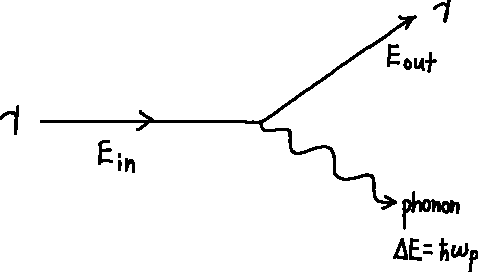
\includegraphics[width=.4\linewidth]{q3-plasmon-scattering}
	\end{figure}
	
	From before we have $\omega_p \propto N^{1/2}$.
	Therefore a plot of $\hbar\omega_p$ against $N^{1/2}$ will be a straight line with gradient $\dfrac{\hbar q}{\sqrt{m \epsilon_0 \epsilon_\infty}}$.
	
	From the graph we then have gradient of $\dfrac{18-7}{3.1-1.2} = \SI{5.789e-11}{\milli\electronvolt \metre^{3/2}}$.
	
	Equating the two expressions then gives
	\begin{align*}
		m &= \frac{\hbar^2 q^2}{\epsilon_0 \epsilon_\infty \, \textnormal{gradient}^2} \\
		&= \SI{3.023e-32}{\kilogram} \\
		&= 0.033 m_e
	\end{align*}
\end{parts}